% !TEX root =  ../main_manuscript.tex 
\section{Simulation Study}
\label{sec:sim_study}
Although we demonstrated personalized schedules for a real patient, we also intend to analyze and compare personalized and fixed schedules in a full cohort. Our criteria for comparison of schedules are the total number of invasive tests planned (burden), and the actual time delay in detecting progression (shorter is beneficial) for each schedule. However, due to the periodical nature of schedules, the actual time delay in detecting progression cannot be observed in real-world surveillance. Hence, instead, we compare personalized versus fixed schedules via an extensive simulated randomized clinical trial in which each hypothetical patient undergoes each schedule. To keep our simulation study realistic, we employ the prostate cancer active surveillance scenario. More specifically, our simulated population is manifested by the joint model fitted to the PRIAS cohort (Web-Appendix~B.3).

\subsection{Simulation Setup}
From the simulation population, we first sample 500 datasets, each representing a hypothetical prostate cancer surveillance program with 1000 patients in it. We generate a true cancer progression time for each of the ${\mbox{500} \times \mbox{1000}}$ patients and then sample a set of longitudinal DRE and PSA measurements at the same follow-up visit times as given in the PRIAS protocol. We then split each dataset into training (750 patients) and test (250 patients) parts, and generate a random and non‐informative censoring time for the training patients. All test and training patients also observe Type-I censoring at year ten of follow-up (current study period of PRIAS). We next fit a joint model of the same specification as the model fitted to PRIAS (Web-Appendix~B.3), to each of the 500 training datasets and retrieve MCMC samples from the 500 sets of the posterior distribution of the parameters. In each of the 500 hypothetical surveillance programs, we utilize the corresponding fitted joint models to obtain the cumulative-risk of progression in each of the ${\mbox{500} \times \mbox{250}}$ test patients. These cumulative-risk profiles are further used to create personalized biopsy schedules for the test patients. For each test patient, we conduct hypothetical biopsies using three personalized biopsy schedules. First using a fixed risk threshold of $\kappa=10\%$. Second, an automatically chosen visit-specific threshold $\kappa^*(v)$. Third, an automatic threshold under the constraint that expected delay is less than 9 months (0.75 years) $\kappa^*\{v \mid E(D)\leq 0.75\}$. We also conduct biopsies according to the currently practiced PRIAS and annual schedules. Successive personalized biopsy decisions~\ref{eq:personalized_decision_grid} are made only on the standard PSA follow-up visits, utilizing clinical data accumulated only until the corresponding current visit time. We maintain a minimum recommended gap of one year between consecutive prostate biopsies~\citep{bokhorst2015compliance} as well. Biopsies are conducted until progression is detected, or the maximum follow-up period at year ten (horizon) is reached. The actual time delay in detecting progression is equal to the difference in time at which progression is detected and the actual (simulated) time of progression of a patient.

\subsection{Results}
Since the simulated cohorts are based on PRIAS, roughly only 50\% of the patients progress in the ten year study period. While we are able to calculate the total number of biopsies scheduled in all $500 \times 250$ test patients, but the time delay in detecting progression is available only for those patients who progress in ten years (\textit{progressing}). Hence, we show the simulation results separately for \textit{progressing} and \textit{non-progressing} patients in Panel~A, and Panel~B of Figure~\ref{fig:simulation_boxplot}, respectively.

For \textit{progressing} patients (Panel~A,~Figure~\ref{fig:simulation_boxplot}), the annual schedule leads to the maximum number of biopsies (Median~3, Inter-quartile range or IQR:~1--6). However, it also guarantees a maximum time delay of one year for all patients. The PRIAS protocol schedules much fewer biopsies (Median~1, IQR:~2--4), but also has a higher time delay (Median~0.74, IQR: 0.38--1.00 years). The personalized schedule based on automatically chosen risk threshold $\kappa^*(v)$ schedules fewer biopsies than PRIAS and has a delay~(Median~0.86, IQR:0.46--1.26 years) slightly higher than PRIAS. The mean delay for schedule $\kappa^*\{v \mid E(D)\leq 0.75\}$ is equal to 0.61 years (Median~0.63, IQR: 0.32--0.88 years) and hence works as expected. Unless the patient progresses within the first year of prostate cancer active surveillance, a delay of up to three years may not increase the risk of adverse downstream outcomes in~\citep{inoue2018comparative,carvalho}. 

The patients who are at the most advantage with the personalized schedules are the \textit{non-progressing} patients (Panel~B,~Figure~\ref{fig:simulation_boxplot}). For all of these patients, the annual schedule leads to 10 (unnecessary) biopsies. The schedule of the PRIAS program schedules a median of 6~(IQR:~4--8) biopsies. In comparison, the schedule based on automatically chosen risk threshold $\kappa^*(v)$ schedules a median of 6~(IQR:~6--7) biopsies, and schedule based on a fixed risk threshold of 10\% schedules only median of 5~(IQR:~4--6) biopsies.

\begin{figure}
\centerline{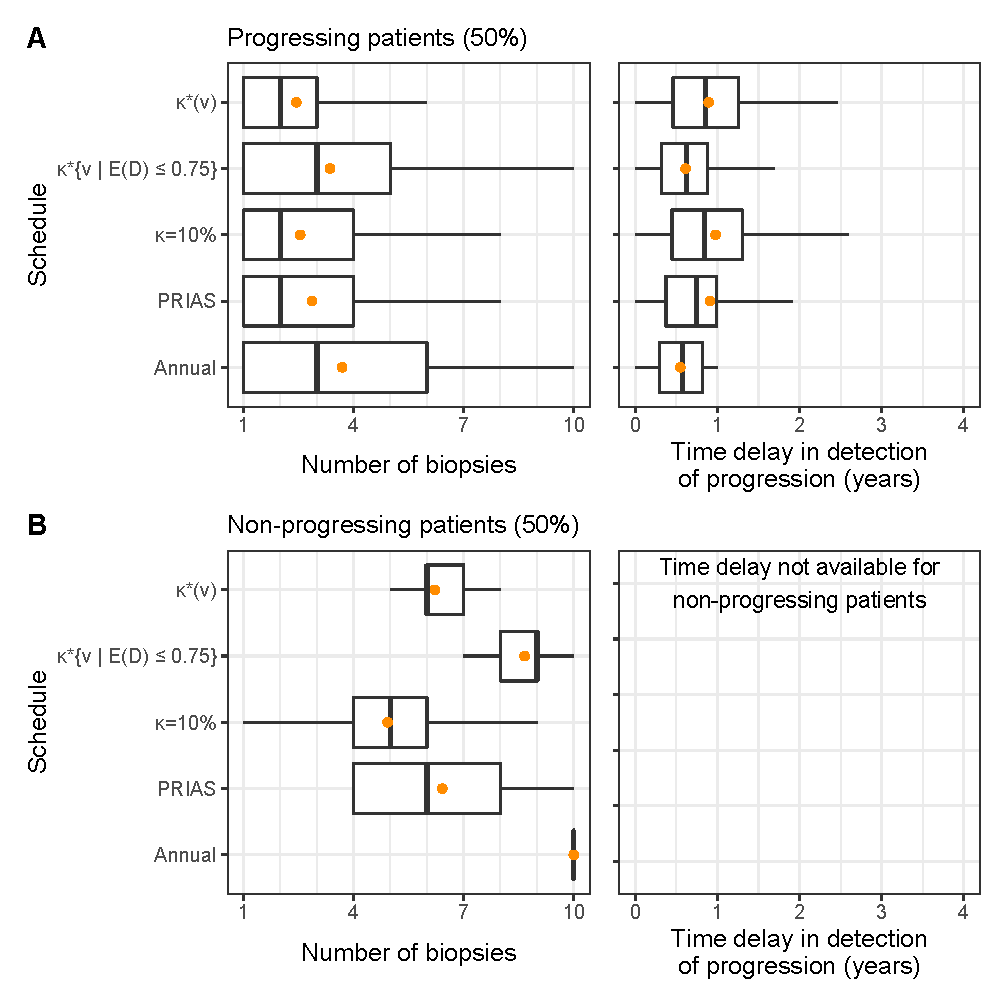
\includegraphics{images/simulation_boxplot.eps}}
\caption{\textbf{Boxplot showing variation in the number of biopsies, and the time delay in the detection of cancer progression} for various biopsy schedules. \textbf{Mean} is indicated by the orange circle. Time delay (years) is calculated as (time of positive biopsy - the true time of cancer progression). Biopsies are conducted until cancer progression is detected. \textbf{Panel~A:} results for simulated patients who obtained cancer progression in the ten year study period (\textit{progressing}). \textbf{Panel~B:} results for simulated patients who did not obtain cancer progression in the ten year study period (\textit{non-progressing}). Types of schedules: ${\kappa=10\%}$ and $\kappa^*(v)$ schedules a biopsy if the cumulative-risk of cancer progression at a visit is more than 10\%, and an automatically chosen threshold~(\ref{eq:kappa_choice}), respectively. Schedule ${\kappa^*\{v \mid E(D)\leq 0.75\}}$ is similar to $\kappa^*(v)$ except that the euclidean distance in~(\ref{eq:kappa_choice}) is minimized under the constraint that expected delay in detecting progression is at most 9 months (0.75 years). Annual corresponds to a schedule of yearly biopsies, and PRIAS corresponds to biopsies as per PRIAS protocol (Section~\ref{sec:results}).}
\label{fig:simulation_boxplot}
\end{figure}